\subsection{Tests}
\label{sec:tests}

To measure the scalability of Ethereum, we prepared some tests to study the
maximal throughput and the size of the blockchain with different configurations.
To study the scalability of one permission-less blockchain system such as
Ethereum one should either rely on
simulation~\cite{bib:securityAndScalabilityPoW} or prepare some tests using
thousand of nodes~\cite{bib:securityAndScalabilityPoW, bib:algorand}. We dispose
neither of a simulation of Ethereum nor dispose of so many resources.
Therefore, we take inspiration from Blockbench~\cite{blockbench}, which
compares the performance and scalability of
Hyperledger\footnote{\url{https://www.hyperledger.org/}} and Ethereum in a
\emph{private} (\emph{permissioned}) scenario, that is, when we consider a
limited number of authenticated nodes.

We tried to use the public available Blockbench
repository\footnote{\url{https://github.com/ooibc88/blockbench}} but we did not
manage to configure it, because of a lot of hard-coded configuration variables
and the lack of a well-written documentation. Thus, we desisted and wrote
our own
system\footnote{\url{https://github.com/gfornari/ethereum-test/tree/benchmark}}.


\subsubsection{Test Configuration}

To keep the configuration easy we opted for a classic master-slave logic. The
master, i.e. the initiator and coordinator of the tests, uses the ssh protocol
to run commands on the remote machines. Similarly to~\cite{blockbench}, we
distinguish between the roles \emph{miner} and \emph{client}. The nodes of the
former type are accountable to generate new blocks while the nodes of the latter
type create and propagate transactions and both verify the blocks\footnote{To
reduce the number of test variables we consider only full nodes. For a list of
node types we refer to~\autoref{sec:node-types}.}. We can assign
multiple roles to a single machine. In this case we run \emph{one distinct geth
instance} for each different role. The coordinator copies the right genesis
block in the test machines.

In each run of test we distinguish at least two phases:
\begin{enumerate*}
  \item the setup and
  \item the test itself.
\end{enumerate*}

\paragraph{Setup phase}
The setup consists in iterating on the test machines twice:
\begin{enumerate}
  \item the required ethash data structures are generated,
  \item the genesis file is used to create the genesis block
  and initialize the ethereum  world state.
\end{enumerate}


\subparagraph{Ethash data structures}
During the setup phase the nodes with the roles miner generate the DAG and the
cache for the first two epochs, while the clients generate only the caches,
because they are required only to validate blocks. We generate the DAGs for the
first two epochs, because ethash uses double buffer of DAGs to grant a smooth
switch between epochs~\cite{bib:dagger-hashimoto}.

\subparagraph{Genesis file}
The genesis file contains useful information to create (deterministically) the
genesis block and the initial state. We report an extract of the genesis file
we used in~\autoref{listing:genesis}. It is simply a JSON file, which specifies
several parameters. Most of them specify directly the attributes of the block
number $0$, which are shown in \autoref{fig:world-state}. Here, we describe
only the fields that are not directly a parameter specification:
\begin{itemize}
    \item \texttt{config}: It describes the network id and the number and hash
    of blocks that marks the entry into force of the Ethereum Improvement
    Proposals (EIP), which indicate incompatible changes in the protocol or
    simply a new version of Ethereum
    \item \texttt{alloc}: It specifies an initial allocation of Ether for the
    accounts\footnote{This possibility has been exploited for the so-called
    Initial Coin Offering (ICO) used by the Ethereum Foundation to obtain fiat
    currency to finance the project.} we use in the tests.
\end{itemize}
Obviously, each node of the network should be initialized with the same genesis
file. Otherwise, the hash of the genesis block differs and the peers cannot
establish a connection with the Ethereum Wire Protocol, as described
in~\autoref{sec:ethereum-wire-protocol}. Thus, the genesis file for the main
network  and the official Ethereum test networks are hard-coded. To create a
new private Ethereum network it is sufficient to use a new genesis file, in
which some parameters are changed. Therefore, in our genesis file we use an
arbitrary network id and nonce, so that packets of different networks are
simply dropped.

\begin{figure}[H]
    \lstinputlisting[caption={An extract of the genesis file used in the tests.}, label=listing:genesis]{./res/code/genesis-file.json}
\end{figure}


Apart from the arbitrary values, that is the id and the nonce, and the data
that perhaps are required by the system do not have influence on the transaction
throughput, the values of some parameters require some justification, that we
provide in the remainder of this paragraph.

The \textbf{timestamp} of the genesis file, that corresponds to the one of the
genesis block, influences the difficulty of the first blocks, and transitively
of all the blocks. Since, for time constraints, we want to run each test for few
minutes we want to avoid sudden decreases in the difficulty due to a too old
timestamp. Therefore, to prevent these unwanted changes in the difficulty value,
during the second loop of the setup phase, the initiator reads its timestamp and
gives it as parameter to the peers\footnote{Before starting the test all the
peers should be configured, therefore using the timestamp of the coordinator
does not assume fine-grained coordinated clocks.}.

As already described in \autoref{sec:consensus:algorithm}, the
\textbf{difficulty} is an adaptive parameter that determines how much effort
should be invested in the creation of a new block. In our tests we used the same
hardware and same operating system in all nodes and for all miners (we
deliberately used only one thread for mining). Therefore to find a suitable
start value for the difficulty for the different configurations we ran a
simulation with one, two, four and eight miners for 24 hours.
\autoref{fig:start_difficulty_raw} shows how the difficulty changed with the
different number of miners. We can notice that in our homogeneous system the
final values of difficulties have a quasi linear dependency with the number of
miners. For the test we took as initial value the median of the last $100$
blocks. These values are represented in~\autoref{table:start-difficulty}. We
reported also the coefficient of variation to show that the values of the last
$100$ blocks are pretty stable.
\begin{figure}
  \begin{center}
    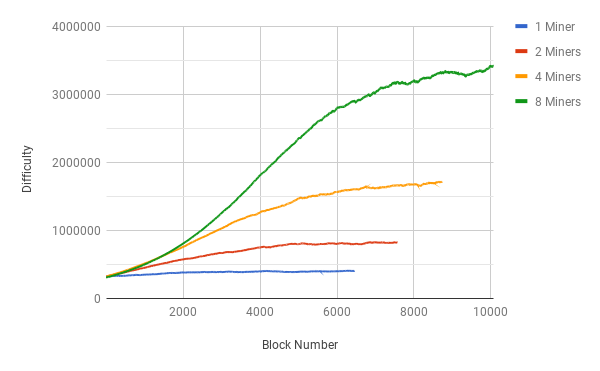
\includegraphics[width=0.8\textwidth]{./res/img/start_difficulty_all.png}
    \caption{The growth of the difficulty in the 24 hour run.}
    \label{fig:start_difficulty_raw}
  \end{center}
\end{figure}

\begin{table}
    \begin{center}
        \begin{tabular}{c | c | c}
            Number of Miners & Difficulty & Coefficient of variation \\
            \hline
            1 &  404559 & 0.0073\% \\
            2 &  821994 & 0.2330\%\\
            4 & 1711150 & 0.1458\%\\
            8 & 3409299 & 0.1742\%\\
        \end{tabular}
        \caption{The median of the last $100$ blocks, value used in the tests as
            start difficulty and the coefficient of variations.}
        \label{table:start-difficulty}
    \end{center}
\end{table}


The \textbf{gas limit} in the genesis block determines the gas limit of the
first block. The gas limit of the subsequent blocks can be determined freely by
the miners but must be contained in a range obtained by summing and subtracting
to the gas limit a portion of itself~\cite{wood2018ethereum}. Thus, in a
relative brief simulation the initial value is fundamental.

\paragraph{Test Phase}
After the setup phase, the real tests begin by starting the execution of the
\texttt{geth} instances on the different machines. The clients emit
transactions that cause simple transfers of values that do not require the
intervention of the EVM, with a predefined release time ($50$ ms), while the
miners starts collecting transactions and creating blocks. The tests are
stopped after a configurable time ($10$ minutes). For each configuration the
tests are repeated a configurable number of times ($5$) because the
probabilistic nature of the Proof-of-Work algorithm and the interaction of many
systems do not guarantee deterministic results.


\paragraph{Concrete Parameters}
We measure the throughput with different number of miners ($1$, $2$, $4$ and
$8$), fixing the number of clients at $16$ with two different gas limits.
The miner machine executes only one \texttt{geth} instance in miner mode, while
the client machines execute two instances in client mode. For our tests we used
the scaleway
platform\footnote{\url{https://www.scaleway.com/}}. We rent $17$ (one master
and $16$ slaves) START1-S servers, which dispose of $2$ X86 64 bit Cores and
$2$ GB of RAM and an internal bandwidth of $1$ Gbit/s, so that the network
would not be a bottleneck. Each server runs Ubuntu 16.04 and has installed,
\texttt{geth} version 1.8.11-stable. During the tests the master acts also as
bootstrap node. We described the role of bootstrap nodes
in~\autoref{sec:network-layer}.

The two tests we conducted differs only for the gas limit in the genesis block,
we wanted to confirm that this value influence the number of transaction
processed as described in \autoref{sec:background}.


\subsubsection{Results}

In this section we report interesting results obtained from the two tests we
conducted. We focused especially on the transaction throughput of the system
but we also report data about the storage needed to run the single systems.

\paragraph{Maximal throughput - Low Gas Limit}
\label{sec:max-troughput}
For this test we used a gas limit of $3141592$, which corresponds to circa
$150 \cdot 21000$. The results are reported in~\autoref{tab:max-troughput}.
We notice that in this case we could not exceed the $10$ transactions per
second and that the number of transaction in each block do not exceed $135$,
although there would be enough space to add other transactions.

\begin{table}[h]
  \centering
  \begin{tabular}{l | cccc}
    & 1 miner & 2 miners & 4 miners & 8 miners \\ \hline
    Avg throughput & 5.37 & 7.17 & 6.73 & 6.65 \\
    Avg blocks & 24.00 & 37.80 & 30.02 & 30.00 \\
    Avg txs per block & 133.77 & 114.69 & 133.61 & 133.15 \\
    Max throughput & 7.18 & 7.76 & 8.17 & 8.67 \\
    Min throughput & 3.68 & 6.83 & 5.91 & 4.91 \\
  \end{tabular}
  \caption{Average throughput and number of mined blocks on 5 runs.}
  \label{tab:max-troughput}
\end{table}


\paragraph{Maximal throughput - High gas limit}
\label{sec:max-throughput-high-gaslimit}
For this test we use a very large gas limit $10500000$ which corresponds to
$500 \cdot 21000$. To give a term of reference, we can consider that
currently (August 2018) the gas limit for the main Ethereum network is circa $8$
million, that corresponds roughly to $381 \cdot 21000$. The results are
summarized in~\autoref{tab:max-troughput-high-gaslimit}. In this case with two
configuration we could exceed the $15$ transactions per second.

\begin{table}[h]
  \centering
  \begin{tabular}{l | cccc}
    & 1 miner & 2 miners & 4 miners & 8 miners \\ \hline
    Avg throughput & 8.17 & 11.55 & 9.02 & 11.07 \\
    Avg blocks & 33.60 & 27.20 & 37.20 & 29.80 \\
    Avg txs per block & 145.25 & 262.98 & 157.15 & 226.32  \\
    Max throughput & 12.55 & 17.50 & 17.77 & 12.525 \\
    Min throughput & 6.82 & 6.83 & 6.83 & 7.14 \\
  \end{tabular}
  \caption{Average throughput and number of mined blocks on 5 runs with high gas limit.}
  \label{tab:max-troughput-high-gaslimit}
\end{table}
